\documentclass{article}
%% Please use 11pt if submitting to AOP
% \documentclass[11pt,twocolumn,twoside]{osajnl}
\usepackage{graphicx}% Include figure files
\usepackage{dcolumn}% Align table columns on decimal point
\usepackage{bm}% bold math
\usepackage{natbib}
\usepackage{physics}



\begin{document}

\section{NV-$^{13}$C Hamiltonian}
The full spin Hamiltonian of the NV-$^{13}$C complex can be written as follow : 
\begin{equation*}
\mathcal{H}=\mathcal{H}_{NV}+\mathcal{H}_{^{13}C}+\mathcal{H}_{HF}
\end{equation*}
Where $\mathcal{H}_{NV}$ is the NV$^-$ spin Hamiltonian described in XX, $\mathcal{H}_{^{13}C}$ is the $^{13}$C nuclear spin Hamiltonian for a $1/2$ spin : $\mathcal{H}_{^{13}C}=\gamma_{n} B I_z$ where $\gamma_{n}=$10.7 MHz/T is the $^{13}$C gyromagnetic ratio, and $\mathcal{H}_{HF}$ is the hyper-fine interaction Hamiltonian : $\mathcal{H}_{HF}= \hat{\mathbf{S}}_{NV} \cdot \mathcal{A} \cdot \hat{\mathbf{I}}_C$.

In the case of first shell $^{13}$C, the hyper-fine tensor $\mathcal{A}$ can be written as \citep{simanovskaia_sidebands_2013} : $$ \mathcal{A} = \begin{pmatrix}
\mathcal{A}_{xx} & 0 & \mathcal{A}_{xz} \\ 0 & \mathcal{A}_{yy} & 0 \\ \mathcal{A}_{zx} & 0 & \mathcal{A}_{zz}
\end{pmatrix} $$

Where $\mathcal{A}_{xx}=190.2(2)$ MHz, $\mathcal{A}_{yy}=120.3(2)$ MHz, $\mathcal{A}_{zz}=129.1(2)$ MHz, and  $\mathcal{A}_{xz}=\mathcal{A}_{zx}=-25.0(1)$ MHz. 

Diagonalizing the total Hamiltonian, we notice that the quantization axis of the nuclear spin (in the limit $\gamma_{n} B << A_{ij}$) is not the same in the manifold of the $\ket{m_s=0}$ state and in the $\ket{m_s=\pm 1}$ states \citep{alvarez_local_2015}, meaning that the nuclear spin is not preserved by the electron spin flip, and giving rise to a splitting of the $\ket{m_s=0} \to \ket{m_s=\pm 1}$ transition in 4 distinct lines when the magnetic field is not aligned with the NV center. \citep{jiang2018estimation}

\section{NV-P1 mutual flip transitions}
Transitions corresponding to a simultaneous flip of the NV$^-$ and P1 spin states, mediated by the dipolar interaction between NV$^-$ and P1 electronic spins, are commonly observed on ODMR spectra \citep{simanovskaia_sidebands_2013} \citep{kamp2018continuous} \citep{alfasi2019detection} \citep{lazda2020cross}. We investigated whether the cross-relaxations processes we observed could be due a three body interaction between two NV centers and a P1 center.

In order for this process to be energy conservative, the P1 transition frequency has to match the energy difference between the $\ket{m_s=0} \to \ket{m_s=-1}$ and $\ket{m_s=0} \to \ket{m_s=+1}$ transitions, giving us the equation \begin{equation}
\label{eq_P1}
\nu^i_{P1}(B)=\nu^{0 \to +1}_{NV}(B)-\nu^{0 \to +1}_{NV}(B)
\end{equation}
Where $\nu^i_{P1}$ is a transition between any of the P1 spin Hamiltonian eigenstates. Note that since we are scanning the magnetic field in the crystalline [100] direction, we do not have to take into account the fours classes of NV centers and P1.

The P1 spin states is defined by its  electron 1/2-spin and its nuclear 1-spin, giving a manifold of 6 spin states. When considering any possible transitions between the 6 eignestates of the P1 Hamiltonian, we have therefore a total of 15 possible transitions, including the nuclear-like transitions which have been observed through mutual flip with NV centers \citep{alfasi2019detection}. 

Basing the numerical values of the P1 Hamiltonian on \citep{lazda2020cross}, we solve eq. \ref{eq_P1} for all possible P1 transitions (see fig. \ref{fig_P1}) therefore giving us all the possible magnetic field amplitude in the [100] direction where we could observe NV-P1 mutual flip transitions. The predicted magnetic field values are 0, 3.89, 5.96, 6.58, 17.90, 28.93, 35.87, 49.44, 81.33, 83.28, 137.52, 154.20 and 246.34 G. None of these values correspond to one of the feature our scans. We then concluded that the Features we observed were not due to NV-P1 mutual flips. 
\begin{figure}
\label{fig_P1}
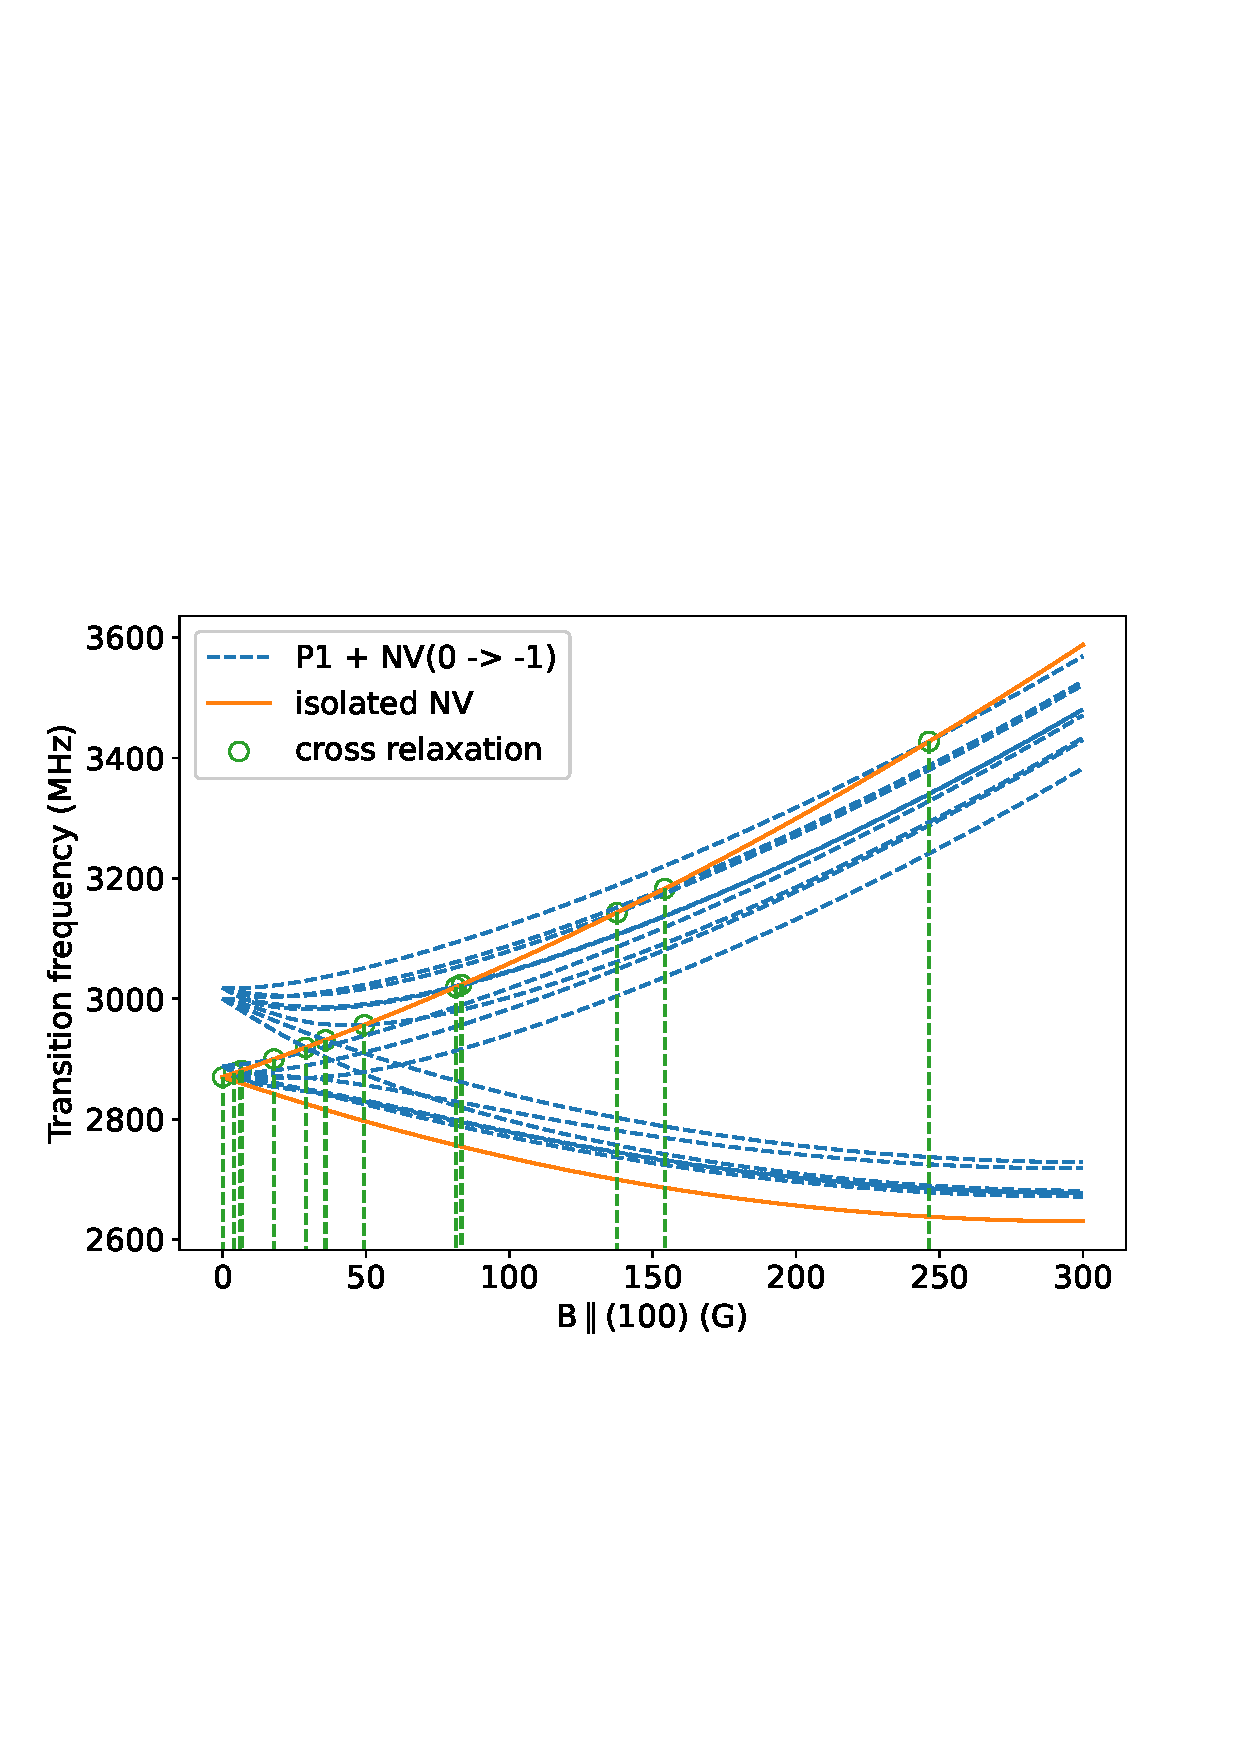
\includegraphics[scale=.6]{Transis_P1}
\caption{Cross-relaxation condition for mutual flip between NV and P1 centers. The orange plain lines correspond to the NV center $\ket{m_s=0} \to \ket{m_s=-1}$ and $\ket{m_s=0} \to \ket{m_s=+1}$ transition frequencies as function of a magnetic field along the [100] crystalline axis, the blue dashed lines correspond to the frequencies of the 15 theoretical transitions of the P1 centers, added to the frequency of the NV $\ket{m_s=0} \to \ket{m_s=-1}$ transition. The green circles correspond to the particular magnetic fields where eq. \ref{eq_P1} is verified, meaning the energy of the P1 transition matches the difference of energy between the two NV transitions.}
\end{figure}
% Bibliography
\bibliographystyle{plain}

\section{Scan in the [111] direction}
\begin{figure}
\label{scan_PL}
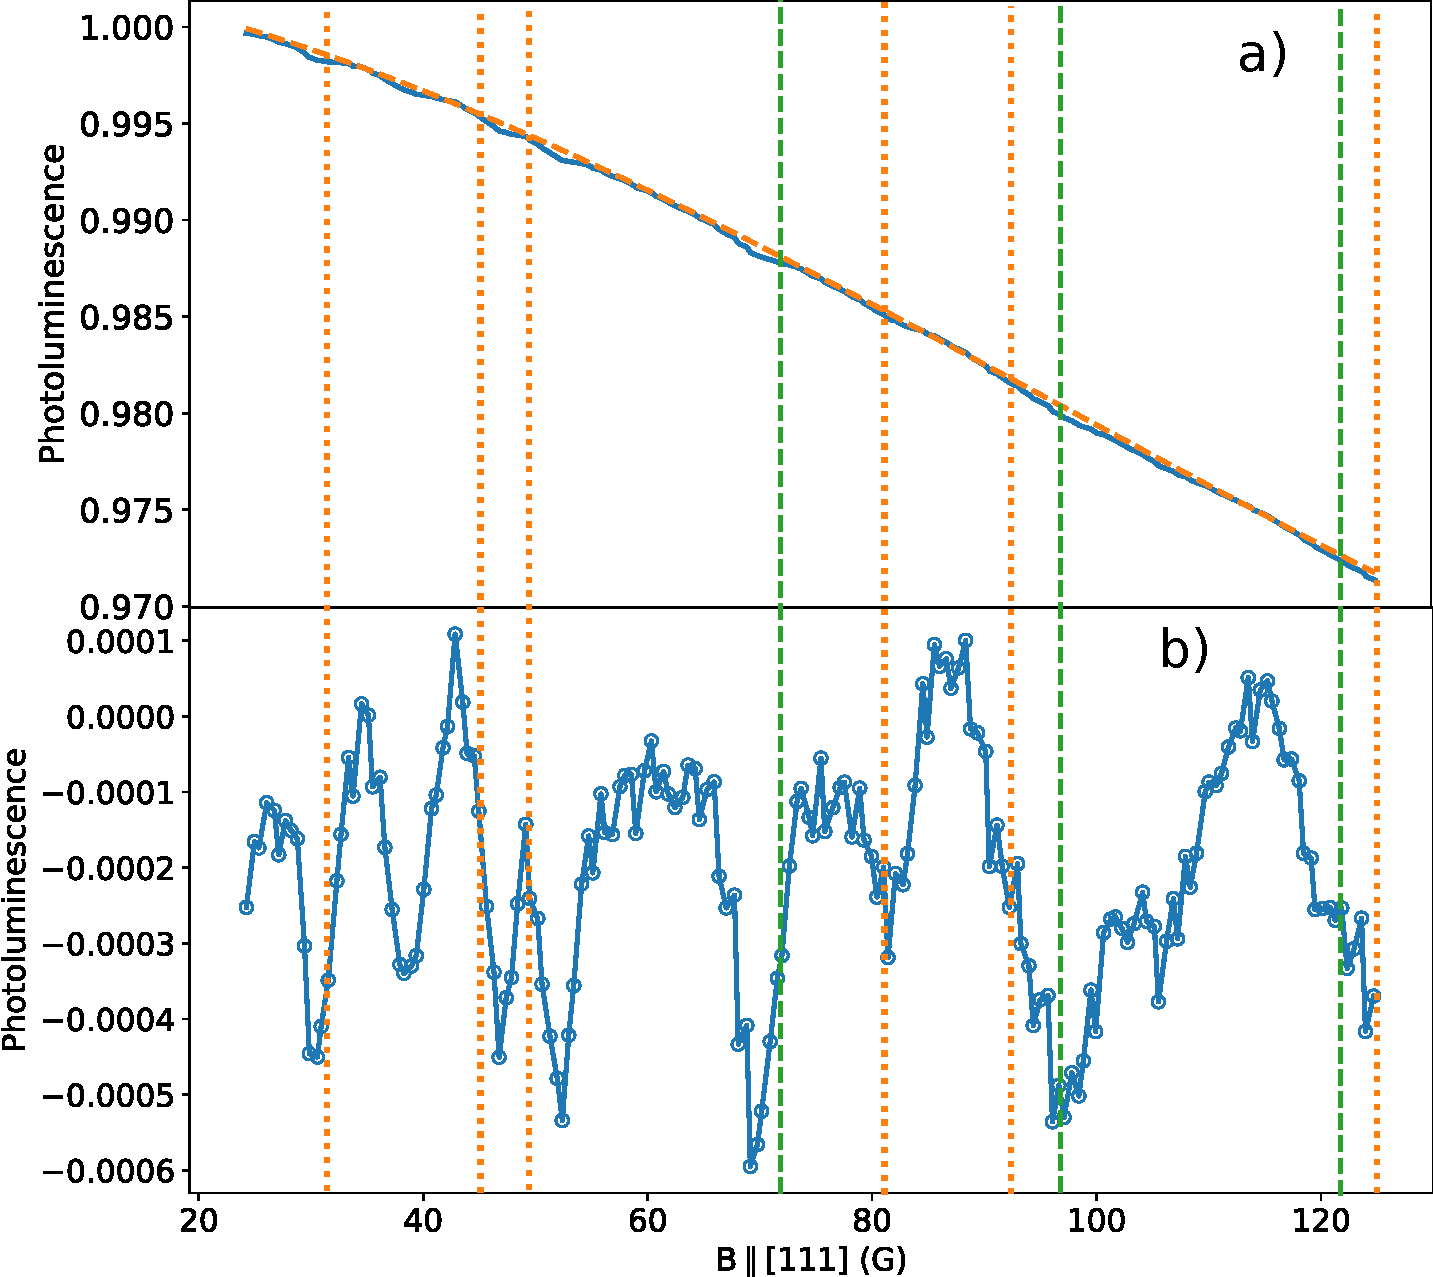
\includegraphics[scale=.48]{scan_111_PL}
\caption{\textbf{a)} Plain blue line : Photoluminescence change as a function of the magnetic field amplitude in the [111] crystalline direction. Dashed orange line : order-4 polynomial fit of the decreasing envelope. \textbf{b)} Subtraction of the previous signal by the envelope fit. The vertical dotted orange lines correspond to the expected cross-relaxations with VH$^-$ and the vertical dashed green lines to the expected cross-relaxations with WAR1.}
\end{figure}
\begin{figure}
\label{transis_VHWAR}
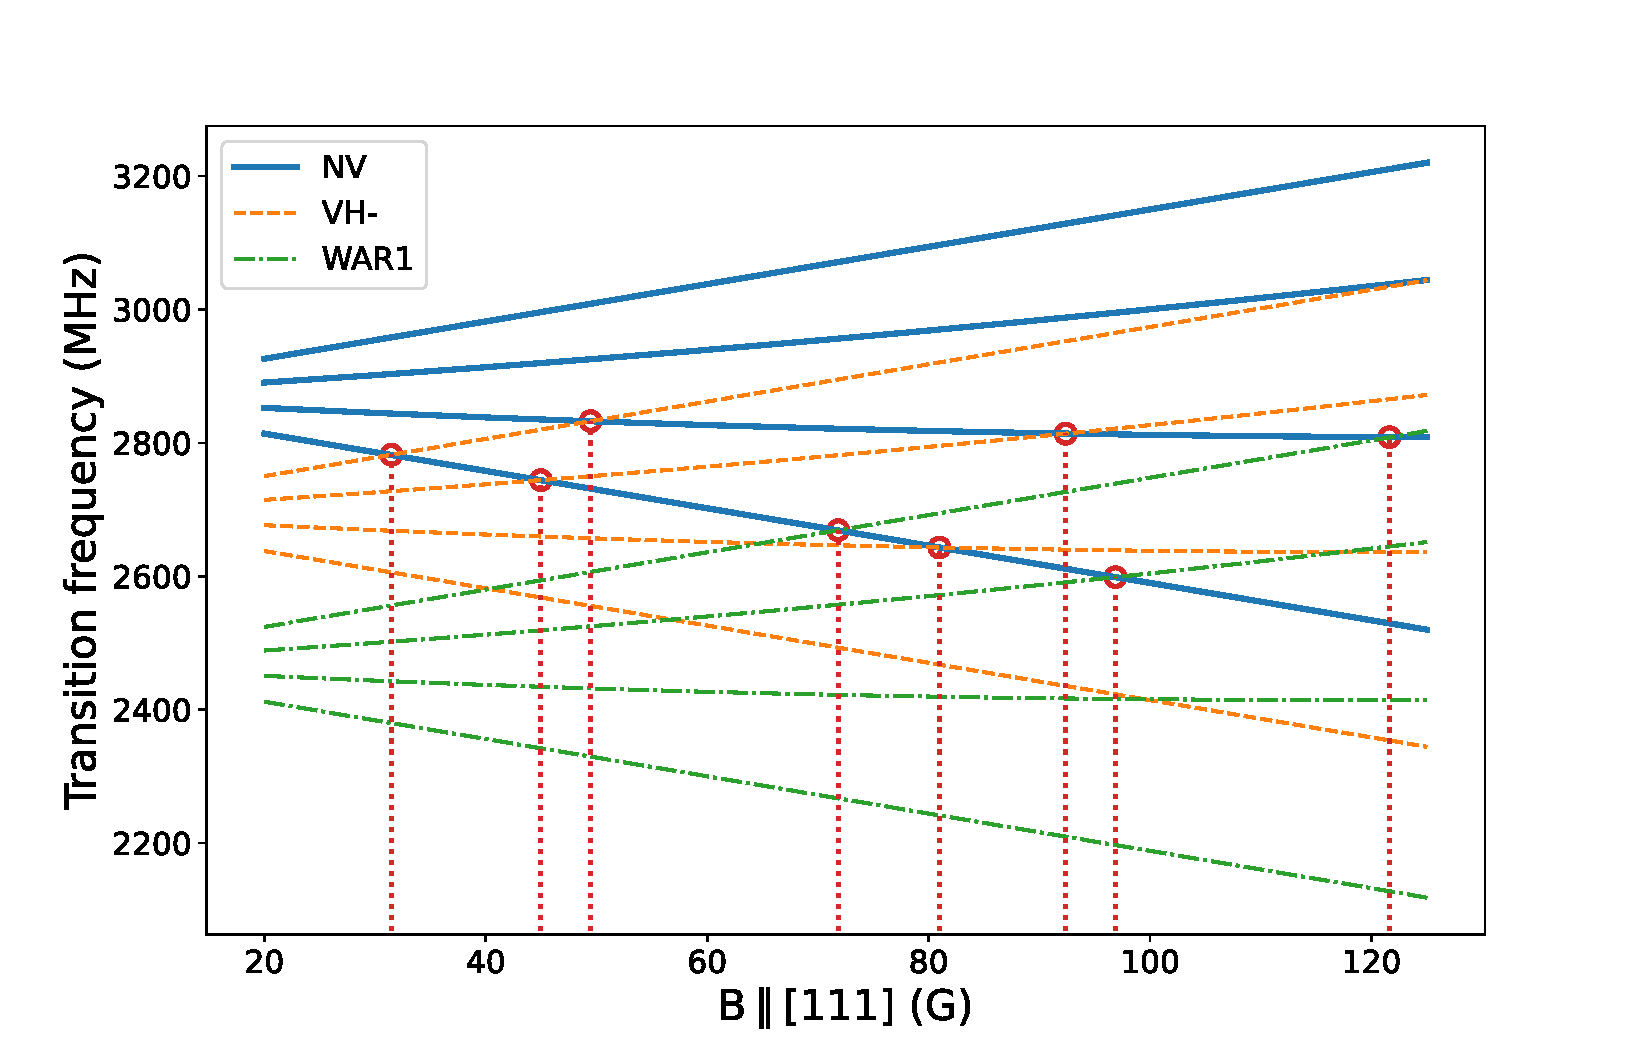
\includegraphics[scale=.48]{Transis_111_VHWAR}
\caption{Predicted transitions frequencies for NV centers (Plain lines), VH$^-$ (dashed lines) and WAR1 (dashdotted lines) when the magnetic field is scanned in the [111] direction. The magnetic field where a transition of the NV center crosses one of VH$^-$ or WAR1 are reported on fig \ref{scan_PL}}
\end{figure}

\begin{figure}
\label{transis_13C}
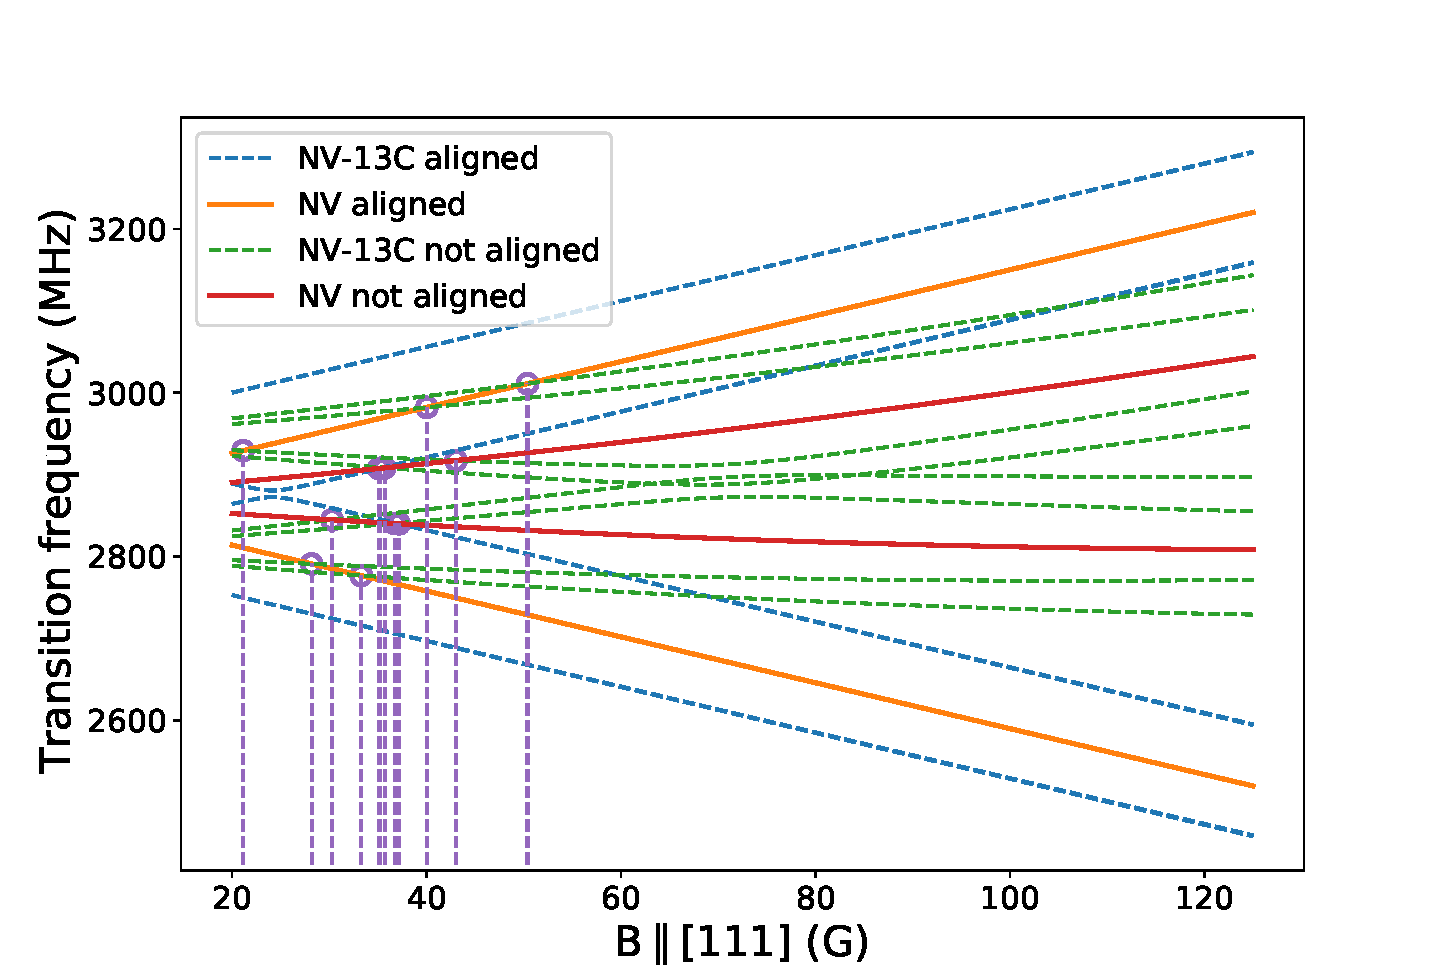
\includegraphics[scale=.55]{Transis_111_13C}
\caption{Predicted transitions frequencies for NV centers (Plain lines) and NV-$^{13}$C complex when the magnetic field is scanned in the [111] direction. Vertical lines represent the various degeneracy conditions.}
\end{figure}

We have performed similar magnetic field scan as presented in Fig.3 of the main text, but this time scanning the magnetic field in the crystalline [111] direction instead of the [100], meaning that this time one class of NV centers is aligned with the magnetic field while the three others are disaligned and degenerated. The results in term of cross-relaxations generally means 4 times as many degeneracy conditions as the [100] case, since the two spins involved in the cross-relaxation process now have two possible orientations, and therefore two separate transitions.

It is then significantly harder to find cross-relaxations signatures, since they are both more numerous and less contrasted than in the [100] case. The experimental results are shown in fig. \ref{scan_PL}. Similarly to fig. 3 of the main text, we have subtracted the envelope associated with the transverse field in order to better see the fine features of the scan. The predicted cross-relaxation conditions between NV centers and VH$^-$ or WAR1 are presented in fig. \ref{transis_VHWAR} and reported on fig. \ref{scan_PL}. While the predicted values do not exactly match the experimental results, it seems like every predicted transition falls in the vicinity of an experimental line. Importantly, it should be noted that, unlike Fig.3 of the main text, the magnetic field was not calibrated with NV ODMR at every field value in this case. Instead we have simply applied an homotethy on the current intensity in the electromagnet to match the field values at the maxima of the scan. This means that the magnetic field of the points of low field value in particular are more susceptible to the non-linearities due to the electromagnet hysteresis cycle.

Finally we have plotted on fig.\ref{transis_13C} the expected cross-relaxations between NV and NV-$^{13}$C complex. It seems that these transitions are too diluted to appear in our experimental scan. The peak at $\sim$37 G in fig.\ref{scan_PL} which in the only peak unpaired with any of the NV-VH$^-$ or NV-WAR1 resonance could come from the resonance between NV and NV-$^{13}$C since they seem particularly dense at this particular field values.
\bibliography{Biblio_CVD-CR}

% Full bibliography added automatically for Optics Letters submissions; the following line will simply be ignored if submitting to other journals.
% Note that this extra page will not count against page length





\end{document}
